\section{Implementation}

There are two parts to this implementation:

\begin{enumerate}
\item The postgress database and populating it.
\item Serving that up via TAP.
\end{enumerate}


No 2. here is well understood  - we have TAP services so we put one in front of the \DB

There are some choices to be made concerning No. 1.

Frossie provided the simple diagram \figref{fig:obsloctap} which captures the ideas.


\begin{figure}
\begin{centering}
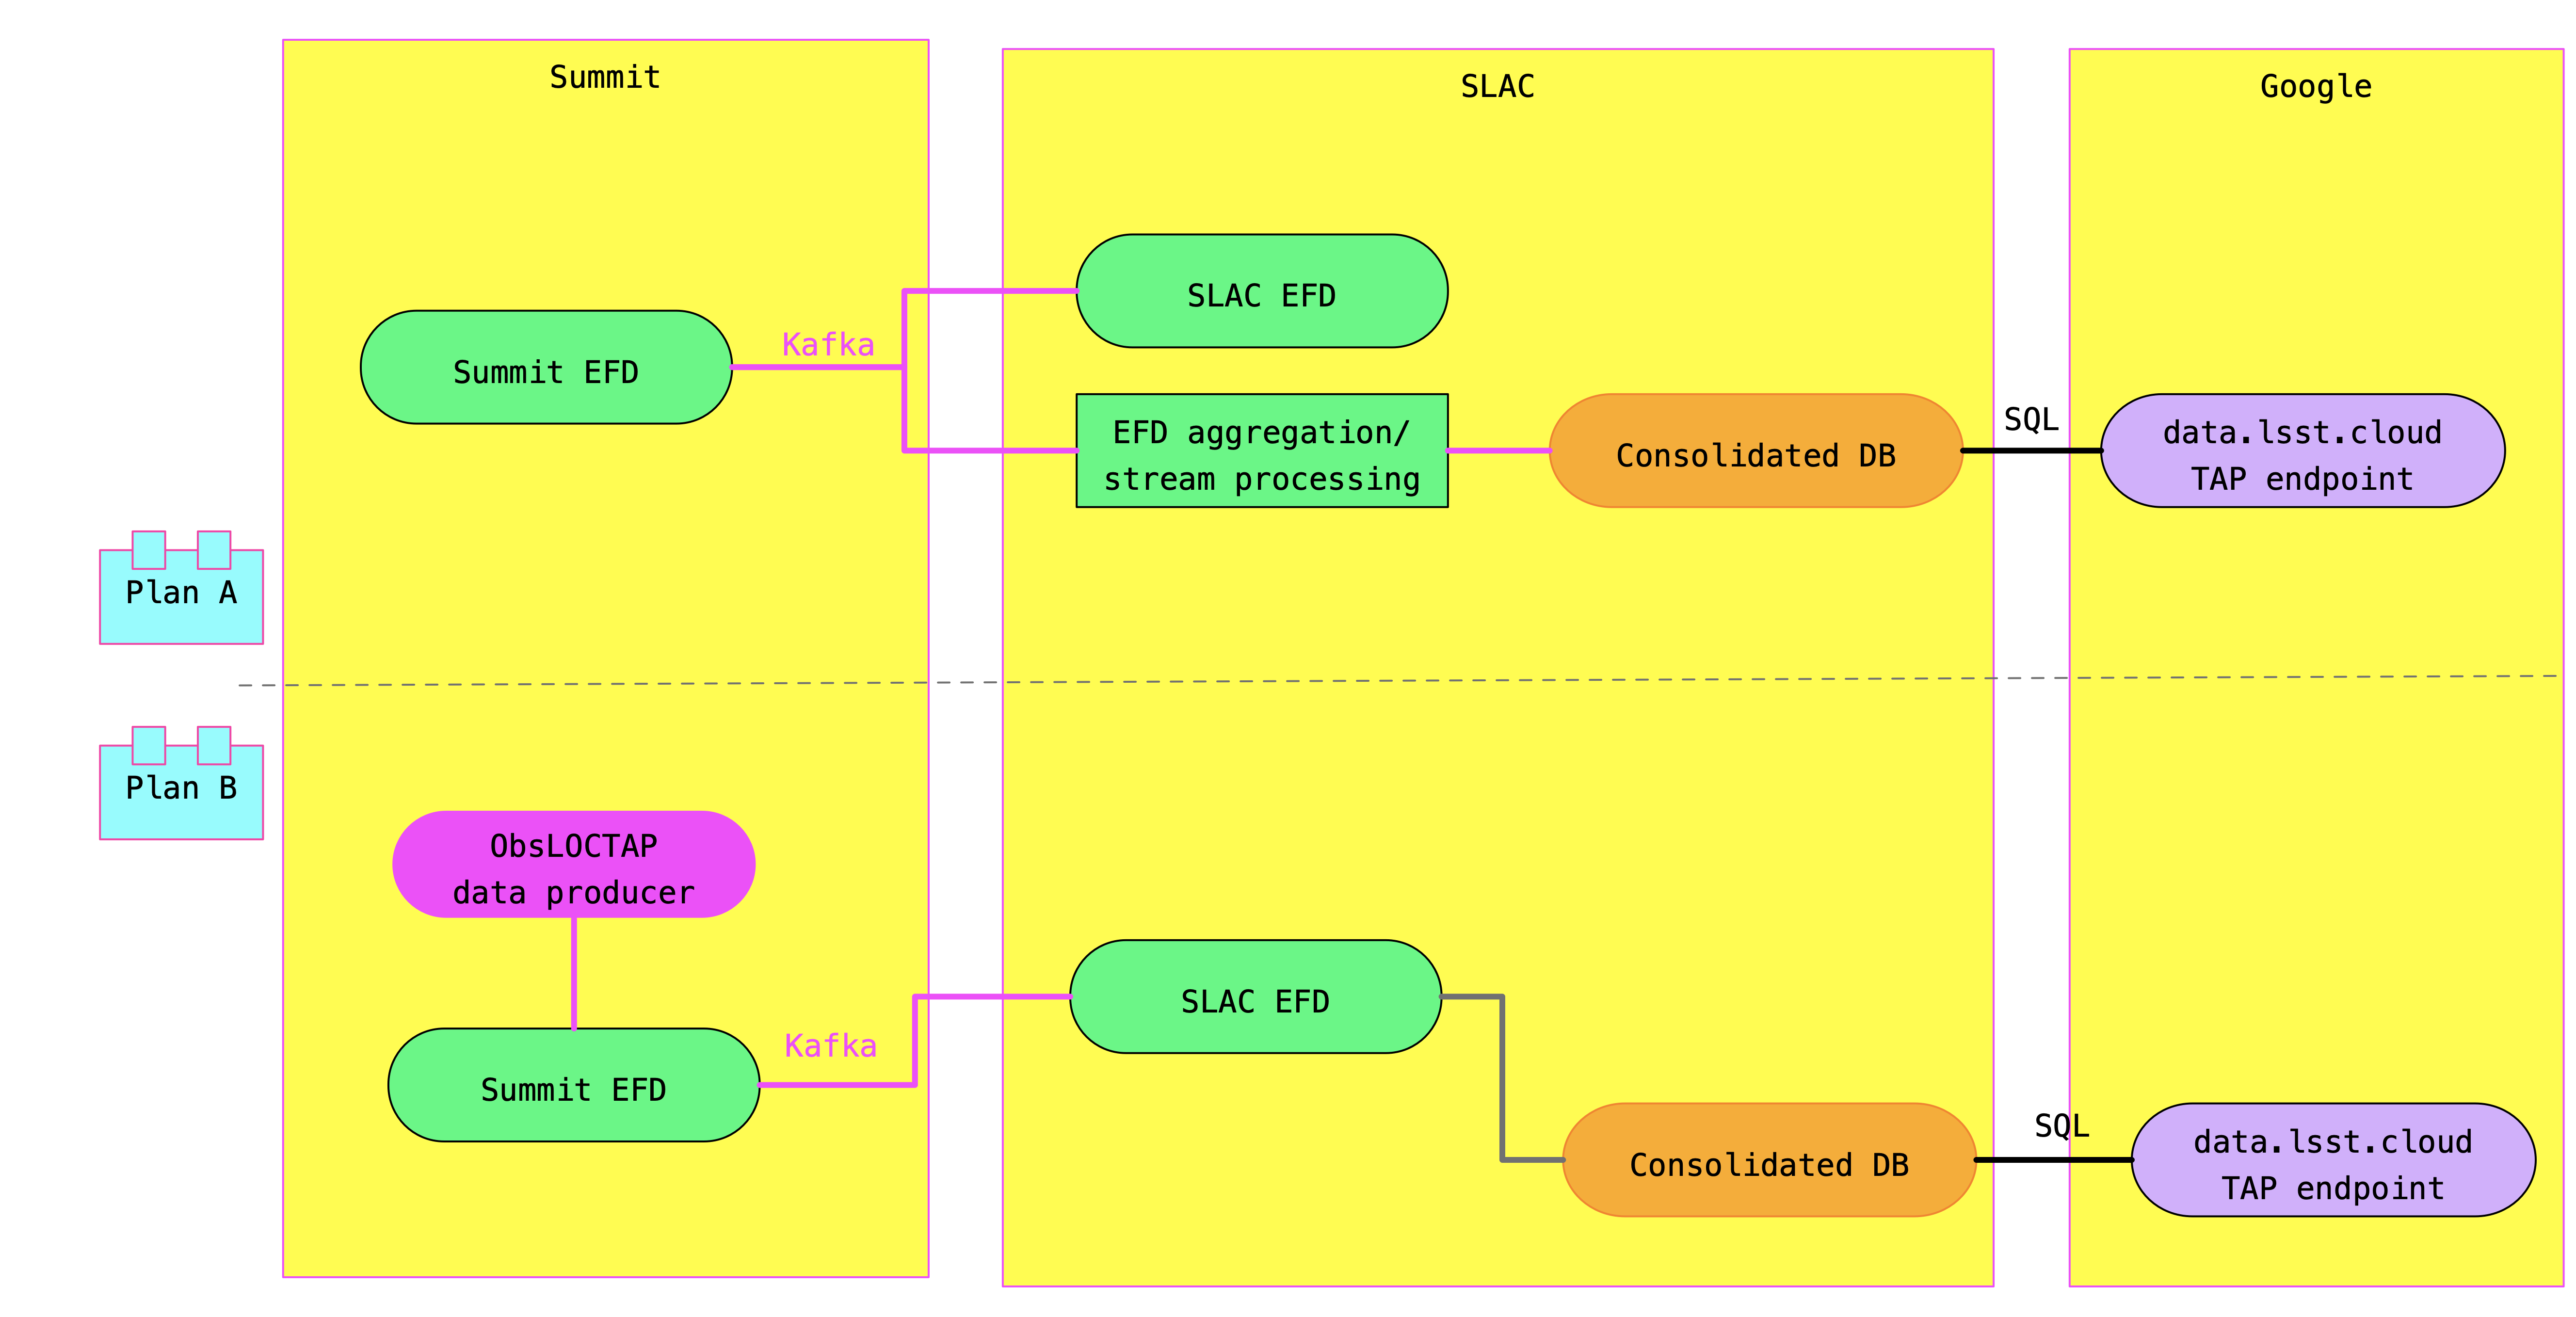
\includegraphics[width=0.8\textwidth]{obsloctap}
	\caption{ Choices on how to populate the postgress database for ObsLocTap.
\label{fig:obsloctap}}
\end{centering}
\end{figure}


\subsection{Create the table}
The yaml was added to {\code sdm\_schema} so Felis may be used to create the schema.

I did not find Felis on pips so I grabbed \url{git@github.com:lsst/felis.git} and installed it with {\tt pip install .}.

I also cloned \url{git@github.com:lsst/sdm_schemas.git}.

This allowed the Felis execution, database login and table creation:i\footnote{ivoa. was removed  from th DDL} \\
\begin{code}
Felis create-all --engine-url="\$engine\_url" --dry-run  sdm\_schemas/yml/obsloctap.yaml > obsloctap.sql

psql -h usdf-butler-session.slac.stanford.edu -U rubin lsstdb1

lsstdb1=> create schema obsloctap;
lsstdb1=> create schema obsloctap\_dev;

SET SEARCH\_PATH = obsloctap\_dev;
\\i obsplan.sql
SET SEARCH\_PATH = obsloctap;
\\i obsplan.sql

\end{code}

Can check the default schema an if  it exists with:
\begin{code}
show SEARCH\_PATH ;
\\dt
\end{code}


\subsection{Populating the \DB}

Initially at least we should try plan A and do all of this at the USDF.
The EFD messages are replicated there so we can pick up the scheduler messages and process them via a stream processor in Kafka (within Sasquatch).

The 24 hour schedule should probably get a new topic to make it distinct from the normal operations - this has to be agreed with scheduler/summit. This will be processed to create schedule entries.

Then we will process {\texttt lsst.sal.Scheduler.logevent\_predictedSchedule } to update/create schedule entries.

Finally we will look at {\texttt lsst.sal.ATHeaderService.logevent\_largeFileObjectAvailable} which will give us a pointer to the header ({\texttt url} field) and using {\texttt astro\_metadata\_translator}  we can get r obsid, exposure\_id, filter and update the \DB appropriately.

\subsection{TAP service}

There is already a ticket \jira{DM-39729} for the creation of the Felis schema.
Another is needed to expose this via tap.

Along the lines of separation of security concerns this would be deployed on the Cloud (US DAC) not in USDF.

Currently the endpoint /schedule will return toe last 1K lines from the Obsplan table as a json file.
This is deployed only on usdfdev as of Dec 2023.
